\documentclass[a4paper,12pt]{article}

\usepackage{prettylatex}
\usepackage{titlepage}
\usepackage{boiboites}
\usepackage{pgfplots}

\top{Université de Technologie de Belfort-Montbéliard}{}
\title{Cours d'IN41}{Chapitre 1 -- Représentation et classification des signaux}
\author{}
\date{Semestre de printemps 2016}

\newboxedtheorem[boxcolor=orange, background={rgb:white,20;green,2;black,1}, titlebackground={rgb:white,15;green,5;black,3},
titleboxcolor = black]{defi}{Définition}{cmpDefi}

\begin{document}

\maketitlepage

\tableofcontents
\pagebreak

\begin{defi}[Signal]
    Un signal est une information relative à une grandeur physique qui évolue dans le temps. C'est une fonction définie telle que :
    \begin{align*}
        S : E & \to \mathbb{R} & \text{ avec } E \subset \mathbb{R} \\
        t & \longmapsto S(t) &
    \end{align*}
\end{defi}

\neverindent

\section{Types de signaux}

Signal analogique : si $E$ est un intervalle réel $\implies$ signal analogique ou continu. \\
Signal numérique : si $E = \mathbb{Z} \implies$ signal discret ou numérique. \\
Signal échantillonné : si $E = \{t_{1}, t_{2}, ..., t_{n}\} \implies$ signal échantillonné.

\section{Analyse et reconstitution des signaux}

\textbf{\'Etape 1} : Reconstituer un signal : déterminer le signal $s$ à partir de la superposition des fonctions élémentaires données pour obtenir une synthèse. \\
\textbf{\'Etape 2} : Analyser un signal : écrire le signal sous forme d'une somme finie ou infinie de fonctions élémentaires.

\section{Classification des signaux}

\textbf{Classification dimensionnelle :} \\
En fonction du nombre de variables

\textbf{Classification réels/complexes :} \\
Si $s(t) \in \mathbb{R} \implies s$ est réel. \\
Si $s(t) \in \mathbb{C} \implies s$ est complexe.

\textbf{Classification déterministe/aléatoire :} \\
Déterministe : évolution prédictible par un modèle mathématique approprié. \\
Aléatoire : évolution non prédictible et non reproductible d'une expérience à l'autre.

\textbf{Classification continu/discret :} \\
Voir 1.1

\textbf{Classification spectrale :} \\
En fonction du domaine de fréquences occupé par son spectre $\Delta F$ (largeur de bande du signal).

$\Delta F = F_{max} - F_{min}$ \\
On considère la fréquence moyenne $F_{moy} = \dfrac{F_{max} + F_{min}}{2}$.

Signaux à bande étroite : $\dfrac{\Delta F}{F_{moy}}$ est une petite valeur. \\
Signaux à bande large : $\dfrac{\Delta F}{F_{moy}}$ est une grande valeur.

\textbf{Classification énergétique :} \\
Il y a deux types de signaux : les signaux à énergie finie ($0 < \omega _{s} < +\infty$) et les signaux à énergie infinie ($\omega _{s} \approx +\infty$).

\begin{defi}[\'Energie et valeur instantanée]
    \'Energie d'un signal :
    \[ \omega _{s} = \int_{-\infty}^{+\infty} ||s(t)||^2 \mathrm{d}t \]

    Valeur instantanée d'un signal :
    \[ s(t_{0}) \text{ (valeur de }s(t) \text{ quand } t=t_{0}\text{)} \]
\end{defi}

\begin{defi}[Valeur moyenne]
    Valeur moyenne d'un signal :
    \[ s_{moy} = \lim_{\Delta t \to +\infty} \dfrac{1}{\Delta t} \int_{t_{0}}^{t_{0}+\Delta t} s(t) \mathrm{d}t \]

    si le signal est $T$-périodique :
    \[ s_{moy} = \dfrac{1}{T} \int_{t_{0}}^{t_{0}+T} s(t) \mathrm{d}t \]
\end{defi}

\begin{defi}[Puissance moyenne]
    Puissance moyenne d'un signal :
    \[ p_{moy} = \lim_{\Delta t \to +\infty} \dfrac{1}{\Delta t} \int_{t_{0}}^{t_{0}+\Delta t} |s(t)|^{2} \mathrm{d}t \]

    si le signal est $T$-périodique :
    \[ p_{moy} = \dfrac{1}{T} \int_{t_{0}}^{t_{0}+T} |s(t)|^{2} \mathrm{d}t \]
\end{defi}

\section{Les signaux classiques}

\textbf{Signal harmonique ou sinusoïdal :} \\
\[ s(t) = \underbrace{A}_{\text{amplitude}} \cos(\overbrace{\underbrace{2\pi ft}_{\text{pulsation }\omega} + \underbrace{\varphi}_{\text{phase à l'origine}}}^{\text{phase instantanée}}) = e^{i2\pi ft}\]

\textbf{Fonctions d'excitation :} \\
Fonctions utilisées pour modéliser des sources d'excitation des circuits électriques.

\paragraph{Rampe unitaire $r(t)$ :}
\[ r(t) =
\begin{cases}
    t & \text{si } t \leq 0 \\
    0 & \text{sinon}
\end{cases} \]

\begin{figure}[!htbp]
	\centering
    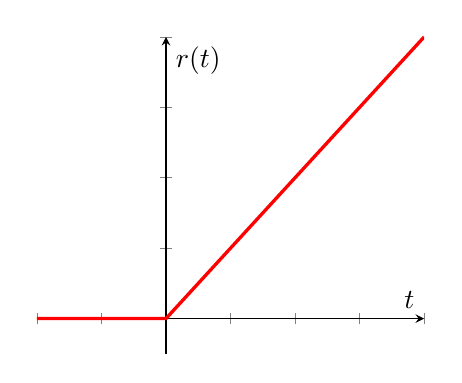
\begin{tikzpicture}
    	\begin{axis}[
            small, axis x line=middle, axis y line=center, xlabel=$t$, ylabel=$r(t)$, xmin=-2, xmax=4, ymin=-0.5, ymax=4,
            xticklabels={,,}, % to hide the numbers on the x axis
            yticklabels={,,} % to hide the numbers on the y axis
            ]
            \addplot+[very thick, red, mark=none, sharp plot] coordinates {(-2,0) (0,0) (4,4)};
    	\end{axis}
    \end{tikzpicture}
	\caption{Représentation de la rampe unitaire $r(t)$}
\end{figure}

\paragraph{\'Echelon unitaire de Heaviside $\Gamma(t)$ :}

\[ \Gamma(t) =
\begin{cases}
    0 & \text{si } t < 0 \\
    1 & \text{sinon}
\end{cases} \]

\begin{figure}[!htbp]
	\centering
    \begin{tikzpicture}
    	\begin{axis}[
            small, axis x line=middle, axis y line=center, xlabel=$t$, ylabel=$\Gamma(t)$, xmin=-3, xmax=3, ymin=-0.2, ymax=2,
            xticklabels={,,}, % to hide the numbers on the x axis
            yticklabels={,,} % to hide the numbers on the y axis
            ]
            \addplot+[very thick, red, mark=none, const plot] coordinates {(-4,0) (0,1) (4,1)};
    	\end{axis}
    \end{tikzpicture}
	\caption{Représentation de l'échelon unitaire de Heaviside $\Gamma(t)$}
\end{figure}

\paragraph{Fonction signe $sgn(t)$ :}

\[ sgn(t) =
\begin{cases}
    1 & \text{si } t > 0 \\
    0 & \text{si } t = 0 \\
    -1 & \text{sinon}
\end{cases} \]

\begin{figure}[!htbp]
	\centering
    \begin{tikzpicture}
    	\begin{axis}[
            small, axis x line=middle, axis y line=center, xlabel=$t$, ylabel=$sgn(t)$, xmin=-4, xmax=4, ymin=-2, ymax=2,
            xticklabels={,,}, % to hide the numbers on the x axis
            yticklabels={,,} % to hide the numbers on the y axis
            ]
            \addplot+[very thick, red, mark=none, sharp plot] coordinates {(-4,-1) (0,-1)};
            \addplot+[very thick, red, mark=none, sharp plot] coordinates {(0,1) (4,1)};
            \addplot+[very thick, red, sharp plot] coordinates {(0,0)};
    	\end{axis}
    \end{tikzpicture}
	\caption{Représentation de la fonction signe $sgn(t)$}
\end{figure}

\paragraph{Fonction fenêtre rectangulaire $rect(t)$ :}

\[ rect(t) =
\begin{cases}
    1 & \text{si } |t| \leq \dfrac{T}{2} \\
    0 & \text{sinon}
\end{cases} \]

\[ rect_{T}(t) = \Gamma(t + \dfrac{T}{2}) - \Gamma(t - \dfrac{T}{2}) \]

Signal utilisé pour observer un signal sur un horizon fini de durée $T$. On dit qu'on applique un fenêtrage rectangulaire sur $s(t)$.

\begin{figure}[!htbp]
	\centering
    \begin{tikzpicture}
        \begin{axis}[
            small, axis x line=middle, axis y line=center, xlabel=$t$, ylabel=$rect(t)$, xmin=-4, xmax=4, ymin=-0.5, ymax=3,
            xticklabels={,,}, % to hide the numbers on the x axis
            yticklabels={,,} % to hide the numbers on the y axis
            ]
            \addplot+[very thick, red, mark=none, const plot] coordinates {(-4,0) (-2,1) (2,0) (4,0)};
        \end{axis}
    \end{tikzpicture}
	\caption{Représentation de la fonction fenêtre rectangulaire $rect(t)$}
\end{figure}

\paragraph{Fonction fenêtre triangulaire $tri(t)$ :}

\[ tri(t) =
\begin{cases}
    1-\dfrac{2}{T}|t| & \text{si } |t| \leq \dfrac{T}{2} \\
    0 & \text{sinon}
\end{cases} \]

\[ tri_{T}(t) = \dfrac{2}{T} r(t + \dfrac{T}{2}) - \dfrac{4}{T} r(t) + \dfrac{2}{T} r(t - \dfrac{T}{2}) \]

\begin{figure}[!htbp]
	\centering
    \begin{tikzpicture}
        \begin{axis}[
            small, axis x line=middle, axis y line=center, xlabel=$t$, ylabel=$tri(t)$, xmin=-4, xmax=4, ymin=-0.5, ymax=3,
            xticklabels={,,}, % to hide the numbers on the x axis
            yticklabels={,,} % to hide the numbers on the y axis
            ]
            \addplot+[very thick, red, mark=none, sharp plot] coordinates {(-4,0) (-2,0) (0,1) (2,0) (4,0)};
        \end{axis}
    \end{tikzpicture}
	\caption{Représentation de la fonction fenêtre triangulaire $tri(t)$}
\end{figure}

\paragraph{Impulsion de Dirac $\delta(t)$ :}

\[ \delta(t) =
\begin{cases}
    1 & \text{si } t = 0 \\
    0 & \text{sinon}
\end{cases} \]

L'impulsion $\delta(t)$ est un opérateur qui extrait la valeur du signal lorsque $t = 0$.

\begin{figure}[!htbp]
	\centering
    \begin{tikzpicture}
        \begin{axis}[
            small, axis x line=middle, axis y line=center, xlabel=$t$, ylabel=$\delta(t)$, xmin=-4, xmax=4, ymin=-0.5, ymax=3,
            xticklabels={,,}, % to hide the numbers on the x axis
            yticklabels={,,} % to hide the numbers on the y axis
            ]
            \addplot+[very thick, red, mark=none, const plot] coordinates {(-4,0) (0,1) (0,0) (4,0)};
        \end{axis}
    \end{tikzpicture}
	\caption{Représentation de l'impulsion de Dirac $\delta(t)$}
\end{figure}

\paragraph{Peigne de Dirac $\dirac_{T}(t)$ :}

\[ \dirac_{T}(t) = \sum_{k=-\infty}^{+\infty} \delta(t - kT) \]

\begin{figure}[!htbp]
	\centering
    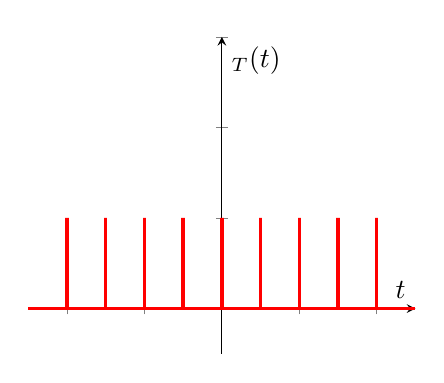
\begin{tikzpicture}
        \begin{axis}[
            small, axis x line=middle, axis y line=center, xlabel=$t$, ylabel=$\dirac_{T}(t)$, xmin=-5, xmax=5, ymin=-0.5, ymax=3,
            xticklabels={,,}, % to hide the numbers on the x axis
            yticklabels={,,} % to hide the numbers on the y axis
            ]
            \addplot+[very thick, red, mark=none, const plot] coordinates {(-5,0) (-4,1) (-4,0) (-3,1) (-3,0) (-2,1) (-2,0) (-1,1) (-1,0) (0,1) (0,0) (1,1) (1,0) (2,1) (2,0) (3,1) (3,0) (4,1) (4,0) (5,0)};
        \end{axis}
    \end{tikzpicture}
	\caption{Représentation du peigne de Dirac $\dirac(t)$}
\end{figure}

\paragraph{Fonction sinus cardinal $sinc(t)$ :}

\[ sinc(t) =
\begin{cases}
    1 & \text{si } t = 0 \\
    \dfrac{sin(\pi t)}{\pi t} & \text{sinon}
\end{cases} \]
\[ sinc(-t) = sinc(t) \]
\[ \forall t = k \in \mathbb{Z}^{*}, sinc(t) = 0 \]

\begin{figure}[!htbp]
	\centering
    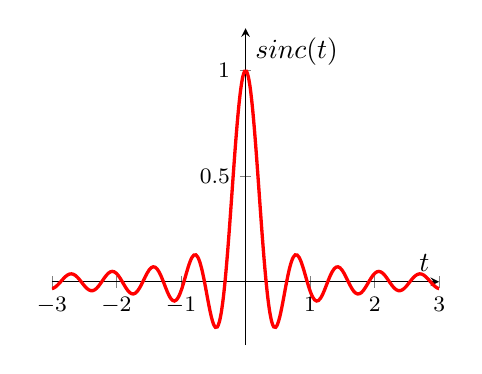
\begin{tikzpicture}
        \begin{axis}[
            small, axis x line=middle, axis y line=center, xlabel=$t$, ylabel=$sinc(t)$, ymin=-0.3, ymax=1.2]
            \addplot+[very thick, red, mark=none, smooth, samples=200, domain=-3:3] {sin(x*180*pi)/(x*pi*pi)};
        \end{axis}
    \end{tikzpicture}
	\caption{Représentation de la fonction sinus cardinal $sinc(t)$}
\end{figure}

\section{Convolution de signaux à temps continu}

Le produit de convolution de deux signaux à temps continu $x(t)$ et $y(t)$ est :
\[ x(t) \otimes y(t) = \int_{-\infty}^{+\infty} x(\nu)y(t-\nu) \mathrm{d}\nu \]

Propriétés : commutativité, associativité, distributivité et élément neutre

\paragraph{Convolution par $\delta(t)$ :}
\[ s(t) \otimes \delta(t-t_{0}) = s(t-t_{0}) \]

\paragraph{Convolution par un peigne de Dirac $\dirac_{T}(t)$ :}
\[ s(t) \otimes \dirac_{T}(t) = \sum_{k=-\infty}^{+\infty} s(t-kT) \]
Convoluer un signal par un peigne de Dirac revient à périodiser le signal à la période T.

\end{document}
